\section{Signalsplejsning} 
\label{Signalsplejsning} 
En opamp forstærker forskellen mellem to spændinger. Det betyder at spændingsforskellen mellem inputterminalerne V+ og V- forstærkes. En ideel opamp kan forstærke en spændingsforskel uendeligt, hvilket medfører at selv en lille spændingsforskel mellem V+ og V- forstærkes uendeligt meget.    
Den ideelle op amp eksisterer kun i teorien, da det antages at kredsløbet er bygget af ideelle komponenter med ideelle egenskaber.
%
\begin{figure}[H]
\centering
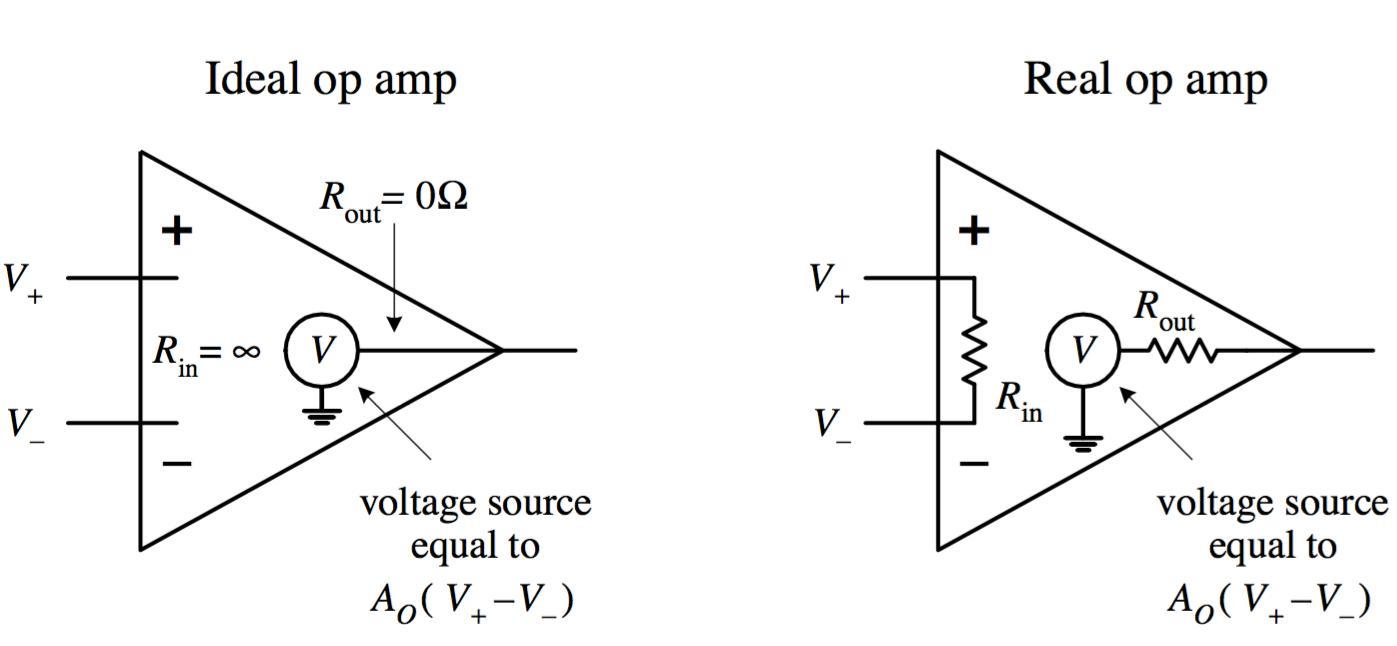
\includegraphics[resolution=300,width=\textwidth]{Figure/Introduktion/IdealRealOpAmp.png}
\caption{manglende figurtekst}
\label{fig:IdealRealOpAmp}
\end{figure}
\noindent
%
Egenskaberne ved en op amp kan siges at være ideelle fordi forstærkningen (Ao) er uendelig, udgangsimpedansen (ZOUT) er 0, indgangsimpedansen (ZIN) er uendelig og der ingen strøm løber mellem V+ og V-. I praksis er det ikke mulig at bygge et sådant kredsløb. En reel op amp har typisk egenskaber der gør den i stand til at forstærke mellem 100.000 og 1.000.000 gange, have en udgangsimpedans mellem 10 og 1K Ohm, en indgangsimpedans mellem 1M ohm og 1T Ohm og en strøm løbende mellem V+ og V- på få nanoampere eller picoampere.\\
%
Alligevel kan det være hensigtsmæssigt at betragte en reel op amp som om den var ideel,  da generaliseringen ikke skaber nogen nævneværdi fejl, men blot gøre det lettere at beregne på kredsløb hvori den indgår.\\
%
Udgangssignalet (VOUT) fra en op amp afhænger af indgangssignalet (VIN=(V+-V-)) og forstærkningen (Ao). Dette kan udtrykkes som VOUT = Ao(V+-V-). Forstærkningen kan derfor udtrykkes som Ao=VOUT/(V+-V-).    
%
\begin{figure}[H]
\centering
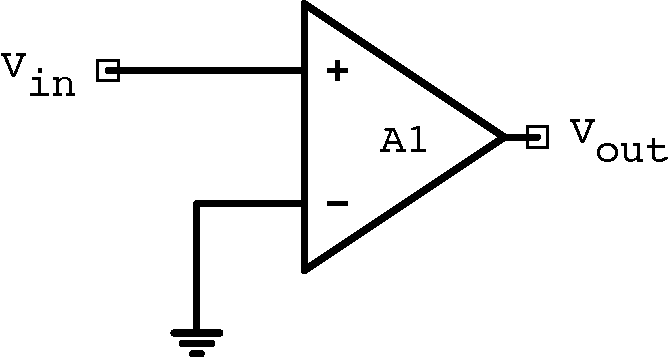
\includegraphics[resolution=300,width=\textwidth/2]{Figure/Introduktion/NonInvertingOpAmp.pdf}
\caption{manglende figurtekst}
\label{fig:IkkeInverterendeOpAmp}
\end{figure}
\noindent
%
I eksemplet ovenfor er den inverterende indgang V- forbundet til 0V og den ikkeinverterende indgang V+ forbundet til VIN. VOUT kan derfor udtrykkes ved at indsætte argumentet for V+ og V- i formlen VOUT = Ao(V+-V-) hvilket giver anledning til omskrivningen VOUT = Ao(VIN-0V) = AoVIN. Forstærkningen kan derfor udtrykkes som Ao=VOUT/VIN. Ideelt set forstærkes VIN uendeligt, hvilket betyder at VOUT er uendelig stor og bærer samme fortegn som VIN.
%
\begin{figure}[H]
\centering
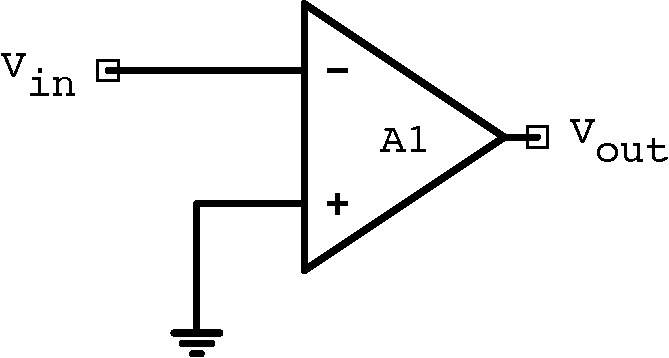
\includegraphics[resolution=300,width=\textwidth/2]{Figure/Introduktion/InvertingOpAmp.pdf}
\caption{manglende figurtekst}
\label{fig:InverterendeOpAmp}
\end{figure}
\noindent
%
I eksemplet ovenfor er det i stedet den ikkeinverterende indgang V+ som forbindes til 0V og den inverterende indgang V- som forbindes til VIN. VOUT kan igen udtrykkes ved at indsætte argumentet for V+ og V- i formlen VOUT = Ao(V+-V-) hvilket giver anledning til omskrivningen VOUT = Ao(0V-VIN) = -AoVIN. Forstærkningen kan derfor udtrykkes som -Ao=VOUT/VIN. Ideelt set forstærkes VIN minus uendeligt, hvilket betyder at VOUT er uendelig stor og bærer modsatte fortegn som VIN.\\
%
En Op amp kan altså ved en simpel kobling hvor et indgangssignal føres til den inverterende indgang og den ikkeinverterende indgang til ground, som vist ovenfor, ideelt inverterer og forstærker indgangssignalsignalet uendeligt. Reelt er det ikke muligt at forstærke signalet uendeligt selvom den ideelle opamp tillader det. Denne uoverenstemmelse ses der dog bort fra da det sjældent er intensionen at forstærke et  signal uendeligt, men derimod at forstærke med en endelig skaleringfaktor, hvorved problemet viser sig at være ubetydende.\\
%
Forstærkningen kan eksempelvis styres ved at koble en opamp så der indgår det der hedder et negativt feedback. Negativt feedback betyder at hele eller dele af udgangssignalet (VOUT) sendes tilbage til den inverterende indgang (V-). V- kan i udtrykket VOUT = Ao(V+-V-) omskrives til at udtrykke den spændning som sendes tilbage via feedback koblingen. Dette gøres ved at indsætte fVOUT på V- plads i udtrykket VOUT = Ao(V+-fVOUT). fVOUT  kan ikke overstige VOUT, men feedbackkoblingen kan ske via en resistor eller en capacitor hvorved det kun er en brøkdel af signalet som sendes tilbage som feedback. Udtrykket kan nu omskrives til VOUT/Ao=(V+-fVOUT). Det smarte ved at tilbagekoble er at V+ og V- hurtigt får samme potentiale, hvilket medfører at (V+-V-)=0. Dette kan forklares under antagelse af at opampen er ideel. En ideel opamp har en uendelig forstækning (Ao), hvilket betyder at udtrykket VOUT/Ao går mod 0. Hvis VOUT/Ao=0, kan udtrykket omskrives til 0=(V+-fVOUT). Med andre ord er der altså ingen spændingsforskel mellem inputterminalerne V+ og V-.
%
\begin{figure}[H]
\centering
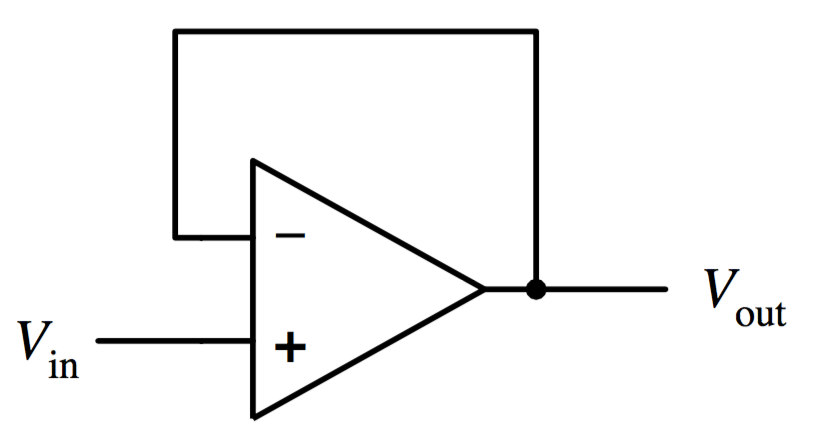
\includegraphics[resolution=300,width=\textwidth/2]{Figure/Introduktion/TilbagekoblingOpAmp.png}
\caption{manglende figurtekst}
\label{fig:TilbagekoblingOpAmp}
\end{figure}
\noindent
%
I eksemplet ovenfor sendes hele udgangssignalet tilbage til den inverterende indgang. Udtrykket for koblingen kan skrives som VOUT = Ao(VIN-fVOUT), hvor f=1, da hele udgangssignalet sendes tilbage til V-. Spædningsforskellen mellem inputterminalerne er 0 i det øjeblik VOUT har samme potentiale som VIN. Opampen forstærker kun forskellen mellem de to spændinger, V+ og V-, som i dette tilfælde hurtigt bliver 0, hvorfor VOUT ikke gå mod uendelig men mod Vin. Med argumentet VOUT=VIN kan udtrykket Ao=VOUT/VIN, skrives som Ao=VOUT/VIN=1, hvilket betyder at forstækningen er 1. Denne kobling kaldes også for en buffer.\\
%
Forstærkningen kan styres ved at det kun er en del af udgangssignalet (VOUT) som sendes tilbage til den inverterende indgang (V-). På den måde vil VOUT forstærkes tilpas nok til at V- får samme potentiale som V+. Dette illustreres i følgende eksempel hvor tilbagekoblingen sker igennem en spændingsdeling.
%
\begin{figure}[H]
\centering
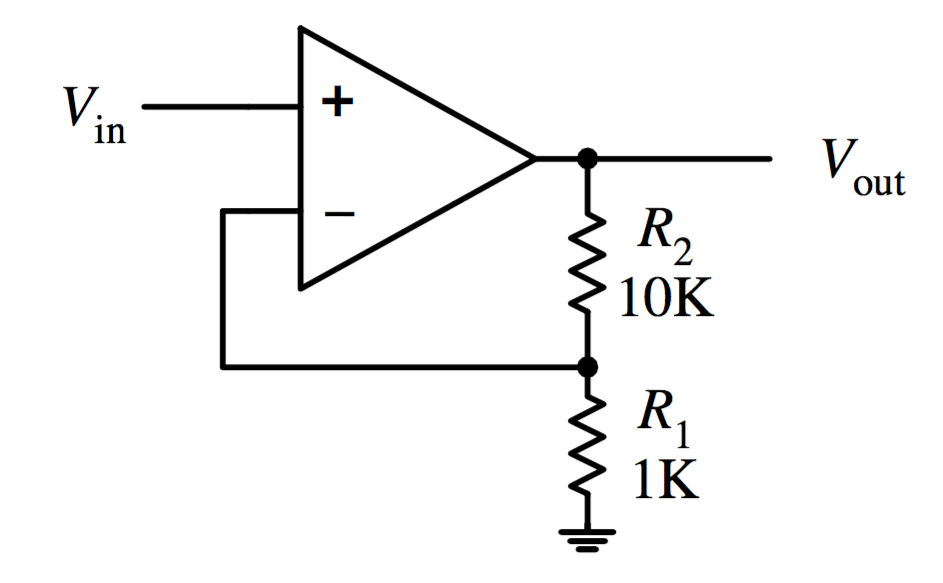
\includegraphics[resolution=300,width=\textwidth/2]{Figure/Introduktion/TilbagekoblingSpaendingsdelingOpAmp.png}
\caption{manglende figurtekst}
\label{fig:TilbagekoblingSpaendingsdelingOpAmp}
\end{figure}
\noindent
%
Spændingsdelingen medfører at $V-=(R1/R1+R2)V_{OUT}$, hvilket i eksemplet kan skrives som $V_-=(1K/1K+10K)V_{OUT}$. V- er altså kun en brøkdel af VOUT. For at V- kan få samme potentiale som V+,må VIN forstærkes indtil VOUT bliver tilpas stor. VOUT skal ifølge udtrykket være 11 gange større end VIN før V- får samme potentiale som V+. Indgangssignalet forstærkes derfor 11 gange, hvilket medfører at udgangssignalet er 11 gange større end indgangssignalet. Udtrykket Ao=VOUT/VIN kan derfor skrives som Ao=11/1=11, hvilket betyder at forstærkingen er 11. (V+-V-)=(VIN-fVOUT)=0 for f=1/11.  
På den måde er det ved hjælp af tilbagekobling, hvor kun en brøkdel af udgangsignalet føres tilbage, muligt at styre hvor meget et signal skal forstærkes i en opamp.\\
%
Ligesom det var muligt at lave en buffer med forstærkningen 1, er det også muligt at lave en inverterende buffer med forstærkningen -1. Dette kan realiseres ved at lave tilbagekoblingen som en del af en spændingsdeler mellem VIN og VOUT, på den inverterende indgang, imens den ikke inverterende indgang (V+) forbindes til ground. Laves en spændingsdeling med to lige store modstande, vil spændingsfaldet være ens over begge modstande, hvorfor der vil ske en halvering af spændingen. Dette er netop grunden til at den inverterende buffer kun invertere signalet uden at forstærke signalet.\\
%
Laves en spændingsdeling med to forskellige størrelser modstande, vil spændingsfaldet afhænge af modstandene. Dette kan ses i eksemplet med den inverterende forstærker herunder.
%
\begin{figure}[H]
\centering
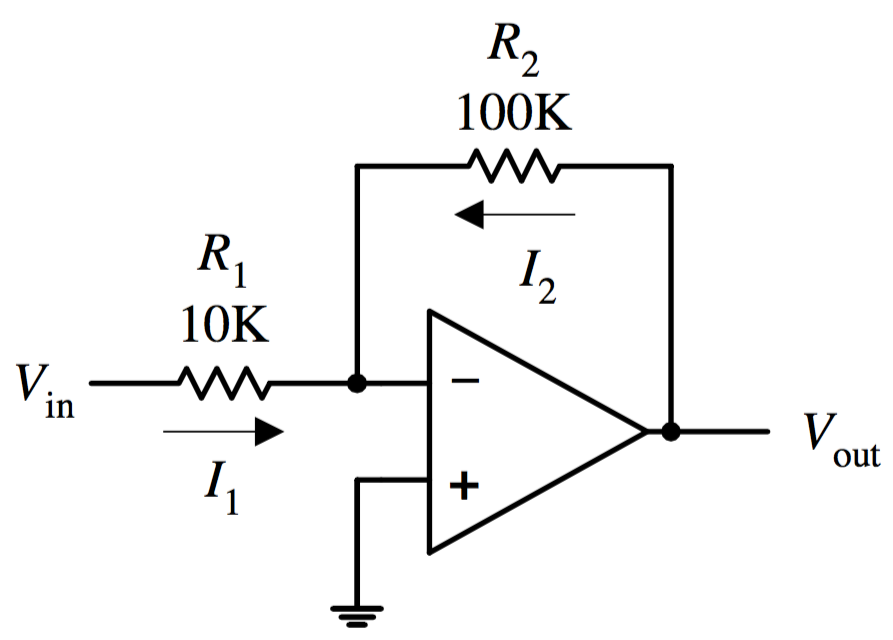
\includegraphics[resolution=300,width=\textwidth/2]{Figure/Introduktion/TilbagekoblingSpaendingsdeling10K100KOpAmp.png}
\caption{manglende figurtekst}
\label{fig:TilbagekoblingSpaendingsdeling10K100KOpAmp}
\end{figure}
\noindent
%
I eksemplet laves en spændingsdeling mellem VIN og VOUT ved hjælp af R1 og R2. Spændingen herimellem danner baggrund for spændingen på den inverterende indgang (V-). Den ikke inverterende indgang (V+) er forbundet til ground, hvilket medfører udtrykket VOUT = Ao(0V-VIN) = -AoVIN. Udtrykket kan også skrives som VOUT/VIN=-Ao hvor -Ao udtrykker forstækningen som resultat af spændingsdelingen mellem R1 og R2. -Ao kan derfor udtrykkes som -R2/R1 og sættes lig med VOUT/VIN. Forstærkningen i eksemplet ovenfor kan derfor udregnes på følgende måde; -Ao=VOUT/VIN= -R2/R1=-100K/10k=-10. VIN forstærkes med andre ord 10 gange. VOUT kan derfor skrives som VOUT =-100K/10k*VIN. På den måde kan en opamp invertere og forstærke med en ønsket faktor, ved hjælp af en spændingsdeling mellem to modstande.\\
%
Dette kan lade sig gøre fordi V+ på opampen er forbundet til ground, hvilket medfører udtrykket (V+-V-)=0 kan skrives som (0V-V-)=0. Udtrykket fortæller at V- har samme potentiale som V+, hvilket kun kan opfyldes ved at V- også er 0V. V- har som udgangspunkt en spænding domineret af VIN, men da opampen invertere og forstærker signalet via en tilbagekobling, kan det siges at potentialet ved VOUT modsvare potentialet ved VIN. Dette kan vises i eksemplet nedenfor hvor en spændingsdeling mellem to spændningsgeneratorer på 1V skaber et potentiale på 0V mellem sig.
%
\begin{figure}[H]
\centering
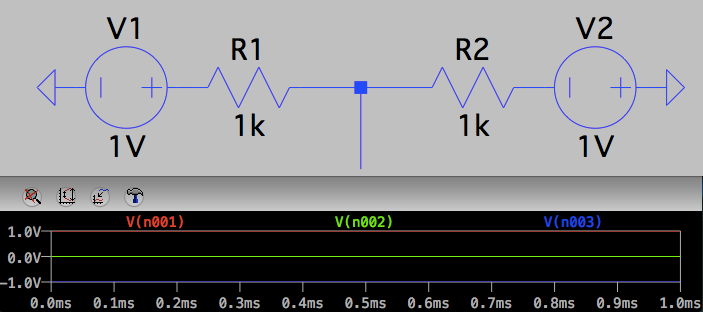
\includegraphics[resolution=300,width=\textwidth]{Figure/Introduktion/PotentialeSpaendingsgeneratorer.png}
\caption{manglende figurtekst}
\label{fig:PotentialeSpaendingsgeneratorer}
\end{figure}
\noindent
%
R1 og R2 er i eksemplet begge 1K Ohm for at spændingsfaldet er ligeligt fordelt over dem. R1 er forbundet til et potentiale på 1V, mens R2 to er forbundet til et potentiale på -1V. Spændningsdelingen mellem modstandene skaber derfor et potentiale på 0V imellem sig, hvilket også kaldes Virtual Ground. Virtual ground skal ikke forveksles med ground, men forstås som en simulering af ground hvor potentialet er 0V.\\
%
Opampen udnytter altså  muligheden for at en spændingsdeling med et positivt potentiale på den ene side og et negativt potentiale på den anden side kan skabe et potentiale på 0V imellem sig. Udtrykket (0V-V-)=0, som fortæller at V- skal have et potentiale svarende til 0V ved V+, kan derfor omskrives til (0V-0V)=0. 
VOUT = Ao(V+-V-)\\
%
SUMMING AMPLIFIER
%
\begin{figure}[H]
\centering
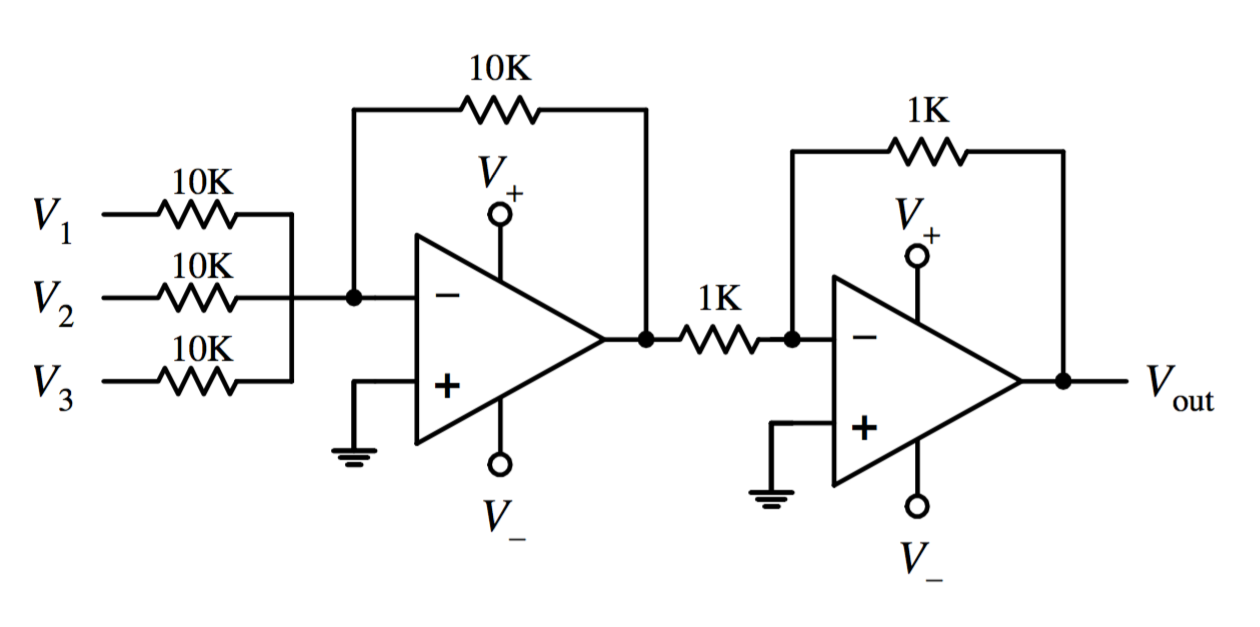
\includegraphics[resolution=300,width=\textwidth]{Figure/Introduktion/SumationskoblingOpAmp.png}
\caption{manglende figurtekst}
\label{fig:SumationskoblingOpAmp}
\end{figure}
\noindent
%